\documentclass[11pt]{article}

\usepackage[utf8]{inputenc}
\usepackage{deauthor}
\usepackage{times,graphicx}

% user packages
\usepackage{todonotes}
\usepackage{pifont}
\newcommand{\cmark}{\ding{51}}
\newcommand{\xmark}{\ding{55}}
\usepackage{multirow}
\usepackage{booktabs}
\usepackage{caption,subcaption}
\usepackage{graphicx}
\usepackage{amsmath}
\usepackage{algorithm}
\usepackage{algorithmic}
\usepackage{hyperref}
\usepackage{amssymb,dsfont}

\title{Enhance Sentiment Classification Using Federated Cross-modal Transfer Learning}

\author{Xueyang Wu$^{\dagger}$
\hspace{2em} Di  Jiang$^{\ddagger}$ 
\hspace{2em} Yuanfeng Song$^{\ddagger}$ 
\hspace{2em} Qian Xu$^{\ddagger}$ 
\hspace{2em} Qiang Yang$^{\dagger}$ \\
$^{\dagger}$ Department of CSE, HKUST, Hong Kong, China \hspace{1em}
\texttt{\small\{xwuba,qyang\}@cse.ust.hk}\\
$^{\ddagger}$ AIGroup, WeBank Co. Ltd., Shenzhen, China \hspace{1em} \texttt{\small \{dijiang, yfsong, qianxu\}@webank.com}}

% unnecessary commands
\usepackage{paralist}
\newcommand{\entity}{\mathcal{E}}
\newcommand{\relation}{\mathcal{R}}
\newcommand{\lang}{\mathcal{L}}
\newcommand{\model}{\mathcal{M}}
\newcommand{\term}{\mathcal{T}}
\newcommand{\kg}{\mathcal{KG}}

  
\begin{document}
\title{Enhance Mono-modal Sentiment Classification With Federated Cross-modal Transfer}

% \author{\IEEEauthorblockN{
% 	 Xueyang Wu\IEEEauthorrefmark{1},
%         Di Jiang\IEEEauthorrefmark{2},
% 	Yuanfeng Song\IEEEauthorrefmark{2},
% 	Qian Xu\IEEEauthorrefmark{2},
%         Qiang Yang\IEEEauthorrefmark{1}\IEEEauthorrefmark{2}}
% \IEEEauthorblockA{\IEEEauthorrefmark{1}HKUST, Hong Kong, China \IEEEauthorrefmark{2}AI Group, WeBank Co., Ltd, Shenzhen, China}
% \IEEEauthorrefmark{1}\{xueyang.wu, qyang\}@connect.ust.hk
% }

\maketitle

\begin{abstract}
Sentiment analysis is a complex process that involves multiple modalities, which can provide more accurate and informative results than using a single modality. Although existing multimodal approaches have shown to be superior to mono-modal sentiment classification, they are not always practical in real-world scenarios where only mono-modal input is available, or where multimodal data is limited due to data scarcity or privacy concerns. To address this issue, we propose a novel approach that enhances mono-modal sentiment classification through federated transfer learning. Specifically, we focus on a practical industrial problem where text and speech data are owned by different affiliations, and we aim to bridge these modalities by sharing a cross-modal feature generator and phone classifier. Our proposed framework also incorporates differential privacy techniques to ensure privacy-preserving cross-modal transfer. Our experimental results on real-world spoken language sentiment classification corpora demonstrate the effectiveness of our proposed framework. We show that our approach can significantly improve the accuracy of mono-modal sentiment classification, even when only a limited amount of data is available.
\end{abstract}



\section{Introduction}\label{sec:introduction}

Sentiment classification has recently attracted significant interest due to its ability to automatically recognize the polarity of human emotional states or attitudes expressed in spoken or written language, which is crucial for improving the user experience in human-machine interaction. Communication among humans involves various modalities, including textual and acoustic content, facial expressions, and body gestures. However, single modality fails to capture sentimental information entirely and leads to inaccurate classification. To address this issue, researchers have proposed multi-modal sentiment or emotion classification approaches that utilize features from different modalities to enhance classification accuracy \cite{li2019acoustic, aguilar2019multimodal}. Text, speech, and vision are three critical modalities for sentiment classification \cite{wollmer2013youtube, rozgic2012ensemble}, and previous research has proposed various fusion strategies to better utilize multiple modalities \cite{zadeh2017tensor, majumder2018multimodal}. Among these modalities, some researchers highlight the importance of text and speech modalities \cite{poria2017context}.

Despite the advantages of multi-modal sentiment classification, two obstacles hinder the application of traditional multi-modal sentiment classification in industry: \textit{data scarcity} and \textit{user privacy}. Collecting multi-modal data is challenging in real-world applications, and mono-modal speech and text data are often the only available options in call centers or text-based conversation systems. Furthermore, annotating parallel multi-modal data is costly and laborious. Moreover, user privacy has become an increasing concern, and many authorities have enacted regulations to protect data and model privacy, such as the EU General Data Protection Regulation (GDPR) \cite{voigt2017the76} in 2018, followed by the US and China.

To address these challenges, we propose a novel federated machine learning paradigm for sentiment classification. Since mono-modal sentimental corpora are more accessible and cost-effective, it is worth enhancing mono-modal sentiment classification if we can leverage multiple corpora with different modalities, leveraging the complementarity of different modalities from multiple sources. To address user privacy concerns when using multiple corpora, we introduce federated learning \cite{yang2019federated}, a collaborative machine learning paradigm where multiple parties jointly learn a global model without exposing their private local data. Our work focuses on scenarios where each party in the federation owns a single-modal sentimental corpus and aims to enhance their sentiment classification performance collaboratively. Further details on related work are provided in Section \ref{sec:related}.

Our proposed framework enables multiple institutes with different modality corpora to collaborate and transfer their knowledge learned from their data in a privacy-preserving manner. The cross-modal transfer is based on the phone sequence, which can be obtained from both text and speech modalities, embedding both phonetic cues and lexical information. Our method takes mono-modal input but utilizes cross-modal transfer to expand the number of modalities. Using the phone sequence as the intermedium between speech and text modality has three benefits: 1) the phone sequence is easy to obtain for both textual and audio input without modifying the existing model significantly; 2) as an intermedium between speech and text, it preserves semantic meaning and speech characteristics; 3) it is straightforward to align the audio pieces and words using the phone sequence at the utterance level. The alignment allows us to enrich the raw text input with speech features learned from the audio modality and embed the acoustic features with semantic meanings learned from the text. During collaborative training, speech-side and text-side institutions join as a federation, only exchanging intermediate model parameters protected by the differential-privacy mechanism instead of sharing raw data or bare model parameters.

\begin{figure*}[!htp]
    \centering
    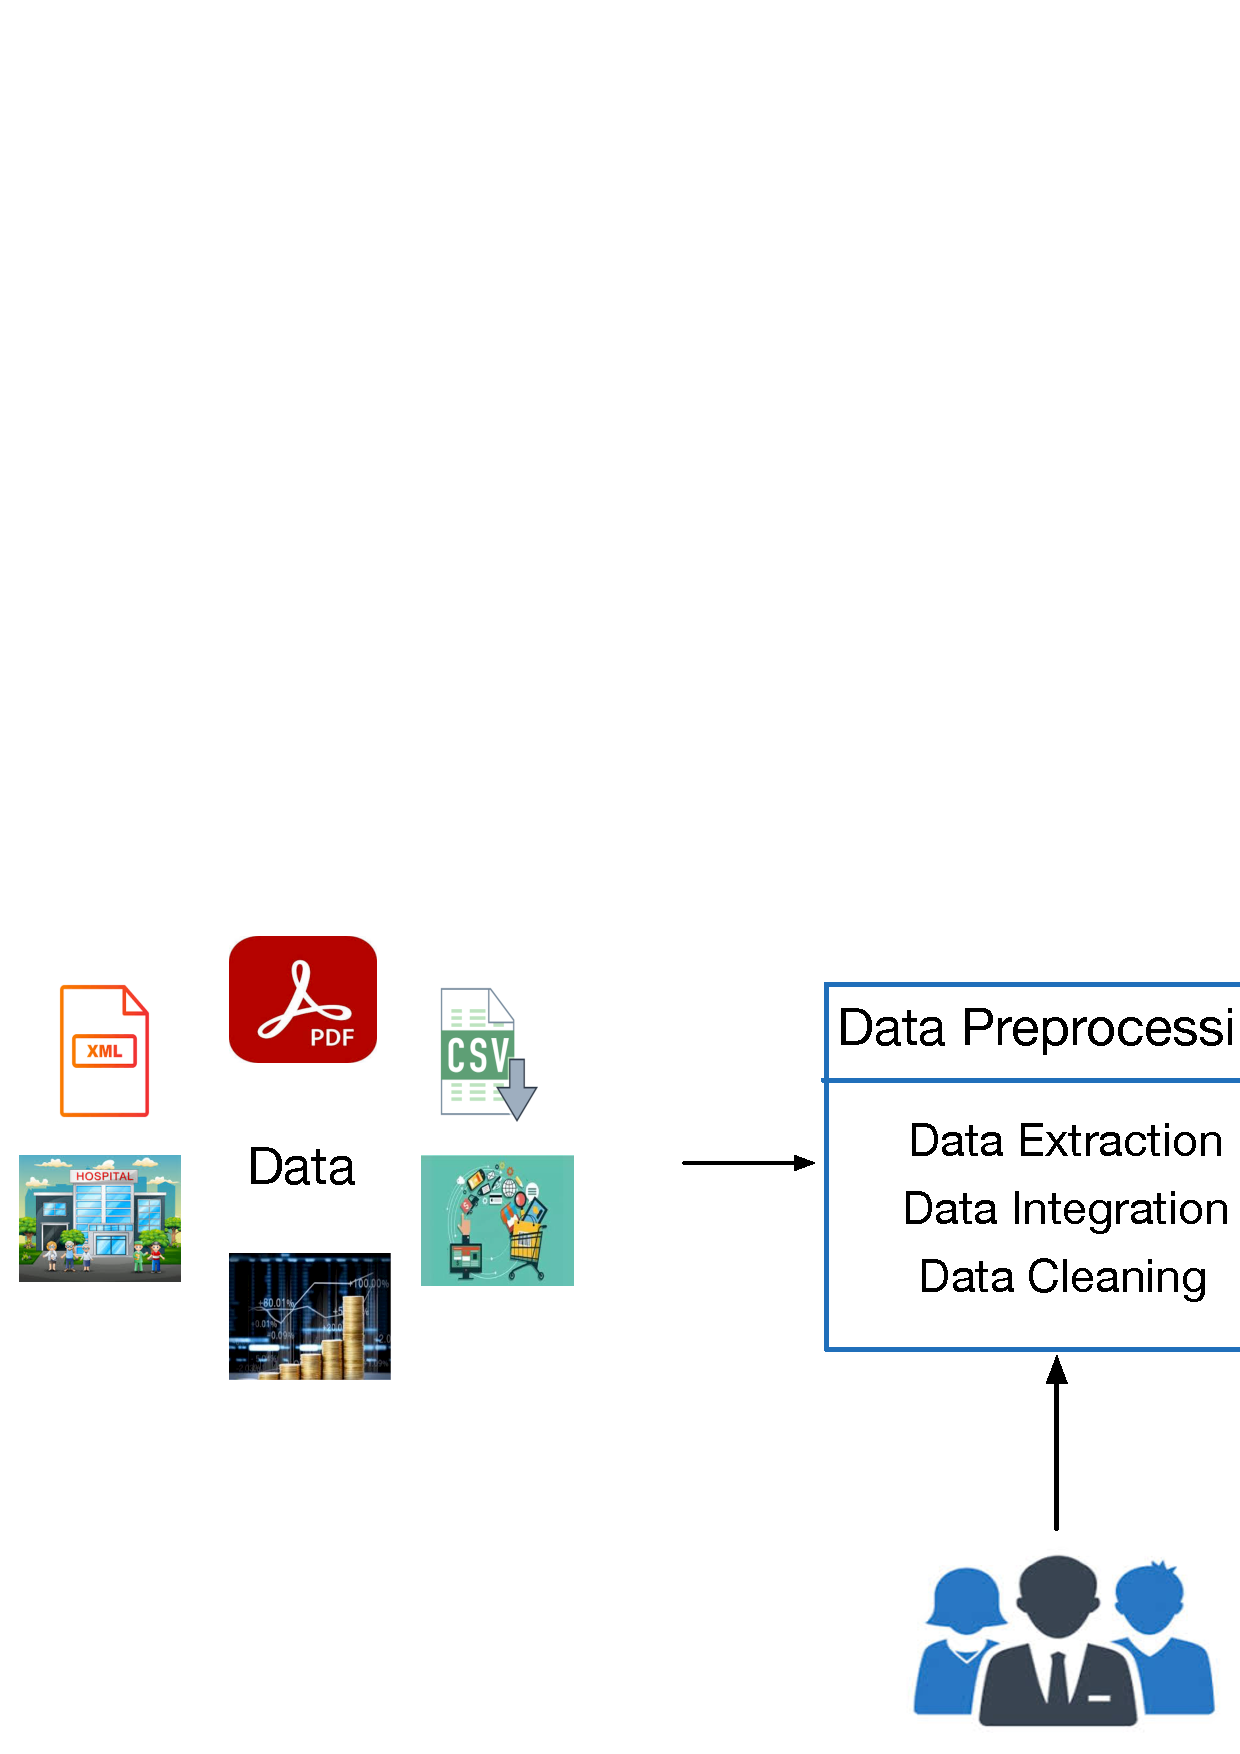
\includegraphics[width=0.9\textwidth, trim={5 5 5 5},clip]{framework.pdf}
    %\vspace*{-7.5mm}
    \caption{The Joint-view of Cross-modal Transfer Learning Framework of Text and Speech module}
    \label{fig:fct}
    \medskip %\vspace*{-2mm}
% \small
% \circled{1} Conduct the mono-modal training of speech sentiment classifier. \circled{2} {Build} the Speech-Phone-Extractor (SPE) from the speech. \circled{3} Share the SPE to the text side. \circled{4} {Setup} phone classifiers and Text-Phone-Extractors (TPEs) on text side and speech side, and conduct local multi-modal training respectively. \circled{5} {Conduct} federated learning over phone-classifiers and TPEs on text-side and speech-side.

\end{figure*} 

% The contribution of this paper is that we propose a novel and practical methodology to improve the mono-modal sentiment analysis by transferring knowledge across different institution of other modality with privacy preservation. Experimental results on real-world spoken language sentiment classification corpora CMU-MOSI and CMU-MOSEI demonstrate the effectiveness of our proposed framework. 

%%\vspace{-3mm}
% \subsection{Contributions}
\section{Related Work}
\label{sec:related}
\subsection{Multi-modal Sentiment Analysis}
Multi-modal sentiment and emotion analysis often involve multiple modalities, such as text, speech, and vision \cite{wollmer2013youtube,rozgic2012ensemble}. Different approaches have been proposed to leverage the information from multiple modalities more effectively \cite{zadeh2017tensor, majumder2018multimodal, poria2016convolutional}, showing that well-designed fusion strategies significantly affect the model performance. Other research works have further explored two-modal sentiment analysis, such as visual-audio fusion \cite{metallinou2008audio,wollmer2013youtube} and textual-audio fusion \cite{li2019acoustic, poria2017context}. These works typically focus on model architecture design or representation extraction. In contrast, our proposed method enhances mono-modal sentiment classification by a novel federated cross-modal transfer framework, where each party in the federation owns data in only one modality.

\subsection{Cross-modal Transfer}
Cross-modal transfer has been used in image classification since 2013 \cite{socher2013zero}. It allows an image classifier to classify a given image class, even if it has not been seen in the training data. Cross-modal transfer leverages the textual description of the object, forces the textual modal and visual modal embedding to map into the same space, and hence allows zero-shot inference with only a textual description of the unseen class. Existing cross-modal transfer methods for sentiment classification often focus on fusing audio and visual modalities based on the correlation between speech and facial expression \cite{albanie2018emotion, dumpala2019audio}. Our approach differs in that it focuses on the semantic complementarity between speech and spoken words. We use phonetic features as an intermediary to connect audio and textual information. For example, when in intense emotion, the pronunciation of words may have distortion, which cannot be observed in the text generated by automatic speech recognition (ASR) but can be captured in the phone sequence.

\subsection{Federated Learning}
Federated learning was first proposed by Google researchers in 2016 \cite{mcmahan2016communication} as a way to learn a global model without explicitly gathering data from different clients. Federated learning has since been extended to various architectures \cite{yang2019federated,yang2020federated}, such as horizontal federated learning, vertical federated learning, and federated transfer learning, with different privacy protection approaches, such as differential privacy \cite{dwork2006calibrating}, homomorphic encryption \cite{rivest1978data}, and multiparty security computation \cite{yao1982protocols}. Among these privacy and security protection techniques, differential privacy has emerged as a widely adapted approach for deep learning because it is practical in terms of computational efficiency. Differential privacy for deep learning is a mechanism that injects deliberately generated noise into the model during the training phase, which offers strong and robust guarantees to bound the probability of revealing raw data under a reasonable threshold. However, there is a tradeoff between high utility and high privacy protection, as injecting more noise into the model leads to less utility. To achieve higher privacy protection, we apply differential privacy to our proposed method, and to maintain high utility, the noises are only injected into a small portion of the model parameters that are shared across parties. Our proposed framework is well-suited for federated learning as it allows two parties to collaborate and share knowledge while keeping sensitive data locally, which effectively relieves the challenges of data scarcity and data privacy in sentiment classification.
\section{Federated Cross-modal Transfer}
%%\vspace{-2mm}


\subsection{Settings and Notations}
\label{sec:settings and notations}

For simplification, we describe our setting as consisting of two parties, and we can easily extend it to the multi-party scenario. We summarize our cross-modal transfer framework in the form of the flow chart in Fig. \ref{fig:fct}, where the red block stands for text modality and the blue one for speech modality. The circled numbers state the general steps of cross-modal joint learning. 

Denote datasets for text-side and speech-side parties as $\mathcal{D}_t=\{\mathbf{w}_i,y_i\}_{i=1}^{N_t}$ and $\mathcal{D}_s=\{\mathbf{s}_i,y_i\}_{i=1}^{N_s}$, respectively, consisting of pairs of the text $\mathbf{w}$ or speech $\mathbf{s}$ and the label $y$, where $N_t$ and $N_s$ are the numbers of training instances of the text-side party and the speech-side party. We use subscripts $(\cdot)_{s}$, $(\cdot)_{t}$ to distinguish where a variable belongs to. As a decentralized federated learning setting, this framework does not involve a central orchestrator, two parties directly set up connections and exchange parameters with each other.

%%\vspace{-4mm}
\subsection{Phone as Intermedium}
%%\vspace{-2mm}
We use phone-level information as an intermedium between text and speech modalities in this work. Phones are the units of speech that constitutes the pronunciation of words. The phone sequence captures the speech pronunciation of a sentence or a word, including the tones and pronunciation variation, such as stress and rhythm, which implies a speaker's sentiment. Phonetic cues have been used to enhance multi-lingual text classification \cite{singh2021classification} and text representation learning \cite{peng2021phonetic}, as phones entail more semantic and sentiment cues than text. On the other hand, the phone sequence is obtainable from both speech and text sides, making it a good bridge to connect the two modalities. For example, a classic DNN-HMM hybrid ASR system can conduct the \texttt{speech-to-phone} transformation to produce the phone sequence of a given speech as the byproduct. The text can also be transformed into a phone sequence with the lexicon representing the ``standard'' pronunciation of the text, denoting this process as \texttt{text-to-phone}.

%%\vspace{-2mm}
\subsection{Federated Cross-modal Transfer Framework}

As shown in Fig. \ref{fig:fct}, our federated cross-modal transfer framework involves two parties and can be summarized in 5 steps. For clarity, we denote the speech-side (blue block) as client-$s$, and the text-side (red block) as client-$t$. Client-$s$ and client-$t$ are two independent institutes that collaboratively enhance their mono-modal sentiment classifier with federated cross-modal transfer with each following the Alg. \ref{alg:s-side} and \ref{alg:t-side} respectively. 


\setlength{\textfloatsep}{0pt}
\begin{algorithm}[ht]
\caption{Federated cross-modal transfer} 
\label{alg:framework} 
\begin{algorithmic}[1]
    \REQUIRE {two parties client-$s$ and client-$t$ with speech sentiment corpus and text sentiment corpus respectively;}
    % \textit{\small // step-1: mono-modal training} \\
    \STATE client-$s$ conducts lines 1-5 in Alg. \ref{alg:s-side} for initialization;
    \STATE client-$t$ conducts lines 1-2 in Alg. \ref{alg:t-side} for initialization;
    \WHILE {\textbf{not} reach maximum rounds}
        \STATE client-$s$ conducts lines 7-12 in Alg. \ref{alg:s-side} and client-$t$ conducts lines 4-9 in Alg. \ref{alg:t-side} \textbf{parallelly};
        \STATE client-$s$ sends ${\phi}_{tpe}^{(s)}, {f}_{p}^{(s)}, {f}_m^{(s)}$ to client-$t$;
        \STATE client-$t$ sends ${\phi}_{tpe}^{(t)}, {f}_{p}^{(t)}, {f}_m^{(t)}$ to client-$s$;
        \STATE client-$s$ conducts lines 13 to update ${\phi}_{tpe}^{(s)}, {f}_{p}^{(s)}, {f}_m^{(s)}$;
        \STATE client-$t$ conducts lines 10 to update ${\phi}_{tpe}^{(t)}, {f}_{p}^{(t)}, {f}_m^{(t)}$;
    \ENDWHILE
\end{algorithmic}
\end{algorithm} % algorithm-1

\textbf{Step 1.} The workflow of the proposed framework starts with client-$s$ training a mono-modal speech sentiment classifier. Then client-$s$ build a Speech-Phone-Extractor (SPE) that embeds the speech signal-level information to phonemes. \textcolor{black}{The speech classifier (${f}_s$) and text classifier (${f}_t$) are implemented with mono-modal models mentioned in Section \ref{sec:imp}.}

\textbf{Step 2.} To avoid missing the focus on our framework, we propose a vanilla SPE practice, which represents a phone with its responding $f_s$ averaged by utterances where this  appears. 

\textbf{Step 3.} Sharing SPE helps client-$t$ build a homogeneous phone classifier as client-$s$, which allows two clients to start federated learning, even though their input modalities are different. 


\textbf{Step 4-5.} Client-$s$ and client-$t$ have different input modalities and mono-modal models while sharing the same phone classifier and the modal-fusion weights. The input of client-$s$ is a piece of speech features $\mathbf{x}$, noted as $\mathbf{s}=\left[\mathbf{x}_1,\mathbf{x}_2,...,\mathbf{x}_T\right]$, extracted from the raw audio wave, where $T$ is the number of frames.  The input of client-$t$ is a sentence, i.e., a word sequence $\mathbf{w}=\left[w_1,w_2,...,w_L\right]$, where $L$ is the length of the sentence. We hence obtains phone sequences from $\mathbf{s}$ and $\mathbf{w}$ with
\begin{equation}
\begin{aligned}
  \mathbf{p}_s &= \texttt{speech-to-phone}(\mathbf{s})~,\\
  \mathbf{p}_t &=\texttt{text-to-phone}(\mathbf{w}).
%   \vspace{-2mm}
\end{aligned}
\label{eq:1}
\end{equation}
Thereafter, each client has two input sequences: speech/text sequence and phone sequence. The speech/text sequence is fed into the mono-modal model, i.e,
\begin{equation}
\begin{aligned}
    \mathbf{o}_s = {f}_s(\mathbf{s})~,~~\mathbf{o}_t = {f}_t(\mathbf{w}).
    % \vspace{-2mm}
\end{aligned}
\label{eq:2}
\end{equation} 

Processing phone sequence is identical for the two clients, so we ignore the superscript of the models ${\phi}_{tpe}^{(\cdot)}, {f}_{p}^{(\cdot)}, {f}_m^{(\cdot)}$. We extract the distributed speech-phone representation $\mathbf{r}_{sp}$ and text-phone representation $\mathbf{r}_{tp}$ of the given phone sequence $\mathbf{p}$,
\begin{align}
    \mathbf{r}_{sp}  = \phi_{spe}(\mathbf{p})~,&~~\mathbf{r}_{tp} = \phi_{tpe}(\mathbf{p}).
\end{align}
The phone representations from two modalities are concatenated and fed into the phone classifier, i.e., 
\begin{align}
    \mathbf{r}_{p} &= [\mathbf{r}_{sp};\mathbf{r}_{tp}]~,~~\mathbf{o}_p = h_p(\mathbf{r}_{p})
\end{align} 
We apply the late fusion (a.k.a., decision-level fusion) strategy \cite{zadeh2017tensor} to combine information from different modalities, i.e,
\begin{equation}
    y = {f}_{m}(\mathbf{o}_{s}, \mathbf{o}_p),~~y = {f}_{m}(\mathbf{o}_{t}, \mathbf{o}_p), \label{eq:7}
\end{equation}




{
We compute the cross-entropy loss with the output $y$ and label $l$ as well as the gradients of parameters through Eq. (\ref{eq:1})-(\ref{eq:7}). The training data of text and speech are store at each client isolatedly, and the two clients only share ${\phi}_{tpe}^{(\cdot)}, {f}_{p}^{(\cdot)}$,  and ${f}_m^{(\cdot)}$ to each other. ${\phi}_{tpe}^{(\cdot)}$ represents ${\phi}_{tpe}^{(s)}$ and ${\phi}_{tpe}^{(t)}$, for simplicity, as well as ${f}_{p}^{(\cdot)}$, and ${f}_m^{(\cdot)}$.  All models are updated with  the Stochastic Gradient Descent optimization algorithm (\texttt{SGD}). To achieve differentially private models, the shared models are updated with the differentially private version of SGD that provides privacy protection of the released model \cite{abadi2016deep}, noted as \texttt{DP-SGD}. In more detail, we inject Gaussian noise \cite{dwork2014algorithmic} to the parameters during optimization. The scale of noise is related to the privacy budget $(\epsilon, \delta)$ indicating the probabilities of leaking privacy. A larger privacy budget allows less model perturbation.

% 把fedavg去掉

Each client conducts local training using their local data, and conducts weighted average over parameters of ${\phi}_{tpe}^{(\cdot)}, {f}_{p}^{(\cdot)}$,  and ${f}_m^{(\cdot)}$. As a  decentralized federated learning scheme, two parties directly exchange differentially private parameters of shared models with each other without the need for a central server \cite{yang2020federated}. Within each party, the weighted averaging follows Eq. (\ref{eq:fedavg}), i.e.,
\begin{equation}
\begin{aligned}
    {\phi}_{tpe}^{(s)}={\phi}_{tpe}^{(t)} &= \frac{\left(|\mathcal{D}_s|\cdot{\phi}_{tpe}^{(s)}+|\mathcal{D}_t|\cdot{\phi}_{tpe}^{(t)}\right)}{\left(|\mathcal{D}_s|+|\mathcal{D}_t|\right)},\\
    {f}_{p}^{(s)}={f}_{p}^{(t)} &= \frac{\left(|\mathcal{D}_s|\cdot{f_p}^{(s)}+|\mathcal{D}_t|\cdot{f_p}^{(t)}\right)}{\left(|\mathcal{D}_s|+|\mathcal{D}_t|\right)}.
    \label{eq:fedavg}
\end{aligned}
\end{equation}
}
% where we ignore the notation of parameters for each model but use the model notation e.g. $\phi_{tpe}$, to represent the parameters of the corresponding model.


% \setlength{\textfloatsep}{0pt}
\begin{algorithm}[!htp]
\caption{DP cross-modal transfer (\textbf{client-$s$})} 
\label{alg:s-side} 
\small
\begin{algorithmic}[1]
    \REQUIRE local training data $\mathcal{D}_s$;
    % \textit{\small // step-1: mono-modal training} \\
    \STATE initialize the local speech classifier (${f}_{s}$);
    \STATE train ${f}_{s}$ with local training data;
    % 	\textit{\small // step-2: build SPE} \\
    \STATE  build SPE ${\phi}_{spe}^{(s)}$ with ${f}_{s}$ according to Alg. \ref{alg:build-spe};
    % \textit{\small // step-3: sharing SPE} \\
    \STATE  share ${\phi}_{spe}^{(s)}$ to client-$t$;
    % 	\textit{\small // step-4,5: federated learning} \\
    \STATE initialize TPE ${\phi}_{tpe}^{(s)}$, phone-classifier ${f}_{p}^{(s)}$, and model-fusion function ${f}_m^{(s)}$;
    \WHILE {\textbf{not} reach maximum rounds}
        \FOR {local training iteration $i$}
            \STATE sample $(\mathbf{s}, \mathbf{l})$ from local training data;
            \STATE compute gradients of ${f}_{s}$, ${\phi}_{tpe}^{(s)}$, ${f}_{p}^{(s)}$, and ${f}_m^{(s)}$ with $(\mathbf{s}, \mathbf{l})$ according to Eq. (\ref{eq:1})-(\ref{eq:7});
            \STATE update parameters of ${f}_{s}$ with \texttt{SGD};
            \STATE update parameters of ${\phi}_{tpe}^{(s)}$, ${f}_{p}^{(s)}$, and ${f}_m^{(s)}$ with \texttt{DP-SGD};
        \ENDFOR
        \STATE send differentially private parameters of ${\phi}_{tpe}^{(s)}$ and ${f}_{p}^{(s)}$ to client-$t$; \\
        \STATE receive differentially private parameters of ${\phi}_{tpe}^{(t)}$ and ${f}_{p}^{(t)}$ from client-$t$; \\
        \STATE update ${\phi}_{tpe}^{(s)}$ and ${f}_{p}^{(s)}$ according to Eq. (\ref{eq:fedavg});
    \ENDWHILE
    \RETURN  {${\phi}_{spe}^{(s)}$, ${\phi}_{tpe}^{(s)}$, ${f}_{p}^{(s)}$, and ${f}_{m}^{(s)}$};
\end{algorithmic}
\end{algorithm} % algorithm-1



\begin{algorithm}[!htp]
\caption{DP cross-modal transfer (\textbf{client-$t$})}
\label{alg:t-side}
\small
% \algorithmfootnote{%\vspace{-10mm}}
\begin{algorithmic}[1]
    \REQUIRE local training data $\mathcal{D}_t$;
    % \textit{\small // step-3: sharing SPE} \\
    \STATE receive ${\phi}_{spe}^{(s)}$ from client-$t$;
    % 	\textit{\small // step-4,5: federated learning} \\
    \STATE  initialize ${\phi}_{tpe}^{(t)}$, ${f}_{p}^{(t)}$, ${f}_m^{(t)}$, and text classifier (${f}_t$);
    \WHILE{\textbf{not} reach maximum rounds}
        \FOR{local training iteration $i$}
            \STATE sample $(\mathbf{w}, \mathbf{l})$ from local training data ;
            \STATE compute gradients of ${f}_{t}$, ${\phi}_{tpe}^{(t)}$, ${f}_{p}^{(t)}$, and ${f}_m^{(t)}$ with $(\mathbf{w}, \mathbf{l})$ according to Eq. (\ref{eq:1})-(\ref{eq:7});
            \STATE  update parameters of ${f}_{t}$ with \texttt{SGD};
            \STATE update parameters of ${\phi}_{tpe}^{(t)}$, ${f}_{p}^{(t)}$, and ${f}_m^{(t)}$ with \texttt{DP-SGD};
        \ENDFOR
        \STATE send differentially private parameters of ${\phi}_{tpe}^{(t)}$ and ${f}_{p}^{(t)}$ to client-$s$; \\
        \STATE receive differentially private parameters of ${\phi}_{tpe}^{(s)}$ and ${f}_{p}^{(s)}$ from client-$s$; \\
        \STATE update ${\phi}_{tpe}^{(t)}$ and ${f}_{p}^{(t)}$ according to Eq. (\ref{eq:fedavg});
    \ENDWHILE
    \RETURN {${\phi}_{tpe}^{(t)}$, ${f}_{p}^{(t)}$, and ${f}_{m}^{(t)}$};
\end{algorithmic}
\end{algorithm} % algorithm-2




%%\vspace{-4mm}
% \subsection{Implementation Details}


% \subsubsection{Phone Classifier}
% The phone classifier  ($h_p$) predict the result using +


\section{Experiments}
%\vspace{-2mm}
\subsection{Experimental Setup}
In this study, we assess the performance of our proposed framework on two public multi-modal datasets, namely MOSI \cite{zadeh2016mosi} and MOSEI \cite{zadeh2018multimodal}, which are available in the CMU Multimodal Data SDK \footnote{\url{https://github.com/A2Zadeh/CMU-MultimodalDataSDK}}.

\subsection{Dataset Description}
\label{sec:data}
Table \ref{tab:data} presents a summary of the datasets, including their size and label distributions. For both datasets, we leverage the training set to train the model and the validation set to fine-tune the hyperparameters. The evaluation of the models is performed on the test set using the hyperparameters chosen through the validation set.


\subsection{Baseline Models and Evaluation Metrics}
\label{sec:monomodal}
To demonstrate the efficacy of our framework, we compare it with two classes of representative mono-modal sentiment classification methods, i.e., {Textual Modal Model} and {Audio Modal Model}, referred to as \textbf{baseline} models. We also perform experiments in the centralized \textbf{oracle} settings. To control for variables, the oracle settings employ the neural network model proposed in this study, but its inputs (text and speech) are aligned per utterance. The oracle settings are ideal but impractical, and they indicate the model's full potential. To further validate the compatibility of our framework with state-of-the-art models, such as BERT~\cite{devlin2018bert} and Transformer, we substitute the mono-modal text model with pre-trained \texttt{BERTLarge} and the speech model with a standard Transformer~\cite{vaswani2017attention}.

All models are tuned with the validation set, and the evaluation metrics are \textbf{F1-scores} reported on the testing sets, which includes four testing sets obtained from two modalities and two datasets.

\begin{table}[!htp]
%%\vspace{-10pt}
\centering
\small
\caption{The statistics of the reference label distribution}%\vspace{1mm}
\begin{tabular}{c|c|c}
\toprule
\textbf{Dataset} & \textbf{MOSI} & \textbf{MOSEI} \\
\midrule
Train & {\textbf{1283} 605:678$^\ddag$} & {\textbf{16331} 8279:8052} \\
Valid & {\textbf{299} 105:124} & {\small \textbf{1871} 939:932}   \\
Test & {\textbf{686} 409:277} & {\small \textbf{5057} 2375:2287} \\
\bottomrule
\end{tabular}
\label{tab:data}
\\{\normalsize $\ddag$ positive-negative count of reference labels}
%\vspace{-10pt}
\end{table}

\subsection{Implementation}
\label{sec:imp}

We provide details of the implementation of our proposed framework, specifically focusing on the phone feature extractor and the acoustic phone feature mapper.

The textual phone feature extractor ($\phi_{tp}$) leverages the Forward-Maximum-Matching (FMM) algorithm to translate an utterance $\mathbf{w}$ to the corresponding phone sequence $\mathbf{p}_t$, with the help of a lexicon.

To recover the acoustic feature from the phone sequence, we propose a concise acoustic phone feature mapper ($\phi_{sp}$). We build a mapper from each context-free phone to an acoustic feature, either from MFCCs or openSMILE \cite{eyben2010opensmile}, following Algorithm \ref{alg:build-spe}. For a given phone sequence $\mathbf{p}_s$, we generate a sequence of acoustic feature vectors $\mathbf{R}_s$. We obtain an utterance vector by taking the mean over $\mathbf{R}_s$.

As we focus on the sentiment classification task, the sentiment labels in the datasets are normalized to positive (intensity $>0$) and negative (intensity $\leq0$). For the acoustic model, we use a handcrafted feature set extracted by openSMILE\footnote{We used the IS09 configuration from \url{https://github.com/naxingyu/opensmile/blob/master/config/}.} \cite{eyben2010opensmile}. This produces a set of features that indicate intensity, loudness, Mel-frequency cepstral coefficients (MFCCs), and pitch. openSMILE extracts 384-dimensional acoustic features for every 100ms-frame. The maximum sequence lengths for words, phones, and acoustic features are all limited to 800.


\begin{algorithm}[!htp]
\begin{algorithmic}[1]
	\caption{Build speech-phone-extractor}              
	\label{alg:build-spe}
		\REQUIRE{an utterance-level acoustic feature extractor ${M}_s$ for speech classification, and a set of speech $\mathbf{X}_s$, a vocabulary of phone $V$}
		\STATE $\mathbf{P}_s = \texttt{speech-to-phone}(\mathbf{X}_s)$;
		\FOR{each phone $p$ in $V$}
		    \STATE  $\mathbf{P}_{sp} = \{\mathbf{p}_s|~p~\in~\mathbf{p}_s,~\forall~\mathbf{p}_s~\in  \mathbf{P}_s\}$;
		    \STATE $\mathbf{R}_{sp} = \{M_s(\mathbf{p}_s)|~\mathbf{p}_s~\in~\mathbf{P}_{sp}\}$;
		    \STATE  $\mathbf{r}_{sp} = \frac{\sum_{\mathbf{r}~\in~\mathbf{R}_{sp}}(\mathbf{r})}{|\mathbf{R}_{sp}|}$;
		    \STATE  $map[p]=\mathbf{r}_{sp}$;
		\ENDFOR
		\STATE $\phi_{spe}(\mathbf{p}):=\left(map[p_j]~|~p=[p_1,...,p_j,...,p_N]\right)$;
		\RETURN{$\phi_{spe}$}
\end{algorithmic}  
\end{algorithm}

We have implemented the Textual Modal Model using a multi-layer bi-directional GRU model \cite{chung2014empirical}, referred to as \textbf{BiGRU}. For the Audio Modal Model, we have used a Convolutional Neural Network \cite{kim2014convolutional} (\textbf{CNN}). Furthermore, to ensure a fair comparison between different settings, we have limited the training iteration at each epoch to 1000.

The proposed framework and baselines have been implemented using PyTorch \cite{paszke2017automatic}, and the differential private algorithm has been applied using PyVacy \cite{waites2019pyvacy}. We have used the differentially private optimizer \cite{abadi2016deep} to train the shared phone classifier. In the differential privacy settings, we have set all $\delta$ to $10^{-5}$, and we have varied $\varepsilon$ to evaluate both protection and performance. All experiments have been conducted on a machine equipped with an Intel(R) Xeon(R) CPU E5-2630, 128 GB RAM, and 4 NVIDIA GeForce GTX TiTian XP GPUs.

\subsection{Experimental Results}


\begin{table*}[!htp]
\centering
% \small
\caption{The F1-score of cross-modal transfer under different privacy budgets}
\label{tab:fct1}
\begin{tabular}{c|c|c|c|c|c|c|c|c}
\toprule
Dataset & \begin{tabular}[c]{@{}c@{}}Baseline \\ \small{(Mono-modal)}\end{tabular} & \begin{tabular}[c]{@{}c@{}}Oracle\\ \small{(Centralized)}\end{tabular} & $\epsilon=1$ & $\epsilon=5$ & $\epsilon=10$ & $\epsilon=15$ & $\epsilon=\infty$ & Avg. \#turn\\ 
\midrule
\small{MOSI-MOSI} & 55.61 & 59.23  & \textbf{57.59} & 57.56  & 57.53  & 57.50   & 56.77 & 3 \\ 
\small{MOSEI-MOSEI} & 62.02 & 66.91 & 63.54 & \textbf{65.84} & 65.82  & 65.71  & 65.73 & 4.8 \\ 
\small{MOSI-MOSEI} & 55.61 & N/A  & 57.65 & 57.53  & \textbf{58.04}  & 58.01  & 57.88  & 7.2 \\ 
\small{MOSEI-MOSI} & 62.02 & N/A & 65.86 & 65.56  & \textbf{65.88}  & 65.86  & 65.58 & 5.8 \\ 
\midrule
\small{MOSI-MOSI}   &  57.42 & 65.23 & \textbf{63.32} & 61.59 & 61.33 & 60.81 & 61.97 &  4.2\\ 
\small{MOSEI-MOSEI} &  68.53 & 70.91 &   70.30 & \textbf{70.54} & 70.51 & 69.98 & 69.73 & 5 \\ 
\small{MOSI-MOSEI}  &  68.53 & N/A &   69.74 & \textbf{70.04} & 69.95 & 69.73 & 69.76 & 6.8 \\ 
\small{MOSEI-MOSI}  &  57.42 &  N/A &   62.01 & \textbf{62.86} & 62.31 & 60.16 & 60.38 & 6.8 \\ 
\bottomrule
\end{tabular}
\end{table*}

Table \ref{tab:fct1} presents the performance of four data settings with varying privacy budgets. The first column provides the details of the four settings in the form of \textit{speech-side} and \textit{text-side} data. In addition to transferring between identical data distributions ({ MOSI-MOSI} and { MOSEI-MOSEI}), we also validate our framework's effectiveness for non-IID and imbalanced distributions ({ MOSEI-MOSI} and { MOSI-MOSEI}), which are more realistic in real-world scenarios \footnote{Note that the training data of speech-side and text-side are neither parallel nor aligned}. The columns from $\varepsilon=1$ to $\varepsilon=\infty$ display the results under different parameter settings. The larger the value of $\epsilon$, the weaker the privacy protection, and the less noise injected into the framework. According to \cite{dpreference}, $\varepsilon$ between 6 and 14 is practical in real-world applications. When $\epsilon=\infty$, the model is trained without any differential privacy protection (e.g., \texttt{FedAvg}).

The results in Table \ref{tab:fct1} show that our federated cross-modal transfer framework enhances performance in all settings. Moreover, we observe that our framework effectively improves the performance of mono-modal inputs to reach the ideal level of aligned multimodal inputs, as compared to the oracle settings. For instance, under-setting $\epsilon=5$, our framework achieves absolute accuracy improvements of 3.82\% and 2.01\% over the baselines in MOSEI and MOSE datasets, respectively. The results also suggest that the improvement is more significant for the side with less training data (as shown in the { MOSI-MOSI} and { MOSEI-MOSI} results from Table \ref{tab:fct1}). The numbers in the last column demonstrate that our framework converges within a few rounds, indicating low network overload. Furthermore, we find that stricter privacy protection does not necessarily lead to performance decreases. In fact, smaller privacy budgets may provide excellent performance, where the injected noise acts as regularization for the model, avoiding overfitting. Importantly, our proposed framework is fully compatible with secure-enhanced schemes such as homomorphic encryption \cite{liu2020secure} and secure multi-party computing \cite{bonawitz2017practical}.


\begin{table*}[!htp]
\centering 
\caption{F1-score of large-scale models under different privacy budgets}
\begin{tabular}{c|c|c|c|c|c|c|c|c}
\toprule
Dataset & \begin{tabular}[c]{@{}c@{}}Baseline \\ \small{(Mono-modal)}\end{tabular} & \begin{tabular}[c]{@{}c@{}}Oracle\\ \small{(Centralized)}\end{tabular} & $\epsilon=1$ & $\epsilon=5$ & $\epsilon=10$ & $\epsilon=15$ & $\epsilon=\infty$ & Avg. \#turn\\ 
\midrule
\small{MOSI-MOSI} & 56.98 & 66.13  & 60.77 & \textbf{60.96}  & 60.32  & 59.53   & 57.17 & 2 \\ 
\small{MOSEI-MOSEI} & 62.01 & 70.22 & 66.14 & \textbf{66.81} & 66.22  & 66.44  & 66.73 & 4.4 \\ 
\small{MOSI-MOSEI} & 56.98 & N/A  & 60.12 & 60.33  & \textbf{61.11}  & 60.01  & 59.88  & 6 \\ 
\small{MOSEI-MOSI} & 62.01 & N/A & 67.16 & \textbf{67.86}  & {66.28}  & 65.98  & 65.38 & 4.6 \\ 
\midrule
\small{MOSI-MOSI}   &  72.26 & 75.32 & \textbf{73.12} & 72.99 & 72.53 & 71.81 & 70.97 &  4.2\\ 
\small{MOSEI-MOSEI} &  74.20 & 78.38 &   76.60 & \textbf{77.45} & 77.23 & 76.89 & 76.73 & 8 \\ 
\small{MOSI-MOSEI}  &  74.20 & N/A &   76.47 & \textbf{77.23} & 76.95 & 76.83 & 76.76 & 10.8 \\ 
\small{MOSEI-MOSI}  &  72.26 &  N/A &   73.20 & \textbf{74.16} & 73.93 & 73.71 & 73.88 & 6.8 \\ 
\bottomrule
\end{tabular}
\label{tab:fct2}
\end{table*}

In order to evaluate the potential of our proposed framework on large-scale models, we replaced the simple CNN speech model and BiGRU text model with a standard Transformer and a pre-trained BERTLarge model, respectively. The results are presented in Table~\ref{tab:fct2}, which shows four settings with two testing sets under different privacy budgets, following the same format as the baseline models. Our findings are interesting. Firstly, we observed that the performance on the text-side testing set is significantly improved by using a pre-trained model. Nevertheless, our federated cross-modal transfer still helps improve the mono-modal performance, approaching the oracle performance. On the other hand, upgrading the speech-side model to a Transformer does not yield a remarkable improvement, and the performance boost provided by our framework remains consistent with the baseline models. Furthermore, we noted that when the models are larger, weaker DP protections are more likely to result in overfitting (as seen in the last few columns of Table~\ref{tab:fct2}).

%  To further depict the enhancement, we depict the relative improvement compared to the baseline with different settings in Fig. \ref{fig:1}, where the solid bars and the dotted bars show the F1-score improvement on the speech modality and the text modality respectively.
 
% \begin{figure*}
%     \centering
%     \includegraphics[width=0.8\textwidth]{figure_1.jpg}
%     \caption{The relative improvement of different settings compared to the baseline}
%     \label{fig:1}
% \end{figure*}



\section{Conclusions}
In this paper, we have proposed a framework for privacy-preserving cross-modal sentiment classification, which leverages the power of multi-modal input features and models trained on different modalities to enhance performance. Our experimental results, both on classic and large-scale models, demonstrate the efficacy of our framework in achieving higher accuracy in sentiment classification, alleviating data scarcity issues, and preserving data privacy for all parties involved. Our work represents a promising initial exploration into knowledge transfer among private modality data, which may hold great potential for improving mono-modal performance via federated cross-modal transfer. However, we acknowledge that this approach also presents challenges, such as privacy protection and communication efficiency, which require further research. We hope that this work will inspire future investigations in this area.

\bibliography{ref.bib}
\bibliographystyle{IEEEtran}



\end{document}
